
\documentclass[11pt]{article}

\usepackage{common}
\usepackage{hyperref}
\title{HW2: Language Modeling}
\author{Jonah Philion \\ jonahphilion@college.harvard.edu \\ \href{https://github.com/jonahthelion/cs287-s18/tree/master/HW2}{github}}
\begin{document}

\maketitle{}
\section{Introduction}

In this problem set, we attempt to classify movie reviews as positive or negative. All models investigated take the form of
$$ x_{i+1} \sim \sigma(W\phi(x_1,...,x_i) + b)$$
where $x_1,...,x_{i+1}$ are word vectors for a sentence and $\sigma$ is the softmax function. The models I try are

\begin{itemize}
\item trigram with linear interpolation
\item NN language model
\item LSTM language model
\end{itemize}

And just for fun
\begin{itemize}
\item Embedding $\rightarrow$ Embedding
\item Fine-tuning ResNet classifier on images of text
\end{itemize}

%This note lays out our expectation for a homework submission in
%\textit{CS287: Statistical Natural Language Processing}. While you do
%not have to follow this template to the letter, we do expect that
%write-ups have a very clear structure and cover all the elements
%described in this note. With this in mind, the burden is on the
%presenter to demonstrate why deviations from the standard are
%necessary.
%
%All write-ups should include a short introduction. In this section you
%should summarize the underlying problem in high-level language and
%describe the extensions that you have decided to propose in your
%implementation. When you describe these extensions you should
%carefully cite the papers of interest. For instance, it will often be
%useful to cite the work seen in class
%\citep{murphy2012machine}. Alternatively, you can also cite papers
%inline, for instance the work of \citet{berger1996maximum}.


\section{Problem Description}
Given 10 consecutive words, we would like to predict the next word.
For all models, a sentence $\boldx_i$ is encoded as a sequence $x_1,...,x_n$ where each $x_j$ is a one-hot vector of length the vocabulary $\mcV$. The model outputs a categorical distribution over the vocabulary $\mcV$. Embeddings $\mcE_d$ map a one hot vector $x_j$ to a dense vector of size $d$. 

%In general, homeworks will be specified using informal
%language. As part of the assignment, we expect you to write-out a
%definition of the problem and your model in formal language. For this
%class, we will use the following notation:
%
%\begin{itemize}
%\item $\boldb, \boldm$;  bold letters for vectors.
%\item $\boldB, \boldM$;  bold capital letters for matrices.
%\item $\mcB, \mcM$;  script-case for sets.
%\item $b_i, x_i$; lower case for scalars or indexing into vectors.
%\end{itemize}
%
%
%For instance in natural language processing, it is common to use
%discrete sets like $\mcV$ for the vocabulary of the language, or $\mcT$ for a
%tag set of the language.  We might also want one-hot vectors
%representing words. These will be of the type
%$\boldv \in \{0,1\}^{|\mcV|}$. In a note, it is crucial to define the
%types of all variables that are introduced. The problem description is the
%right place to do this.
%
%% NLP is also
%% full of sequences. For instance sentences, $w_1, \ldots, w_N$, where
%% here $N$ is a constant length and $w_i \in \mcV$ for all
%% $i \in \{1, \ldots N\}$. If we pretend sentences are all the same
%% length, we can have scoring function over sentences,
%% $s : \mcV^N \mapsto \reals$.  One might be defined as:
%
%% \[ s(w_1, \ldots, w_N) = \sum_{i = 1}^N p(w_i | w_{i-2}, w_{i-1}), \]
%
%% \noindent where $p$ is the bigram probability, which we will cover later in the class.

\section{Model and Algorithms}

All models are trained on the \href{http://aclweb.org/anthology/J93-2004}{Penn Treebank}. For models requiring gradient descent, training loss and validation loss are recorded in real time with \href{https://github.com/facebookresearch/visdom}{visdom}. Final Mean Average Precision (MAP) is calculated on a validation set. 

\subsection{Evaluation}
\begin{enumerate}
\item All models assume a vocabulary of $10000$ and have a \ttfamily{predict} function which given a batch of sentence fragments outputs an array containing the probabilities for the next word for all batches.

\item All models are tested with the same evaluation function. The function evaluates the model on batches of size 67 of bptt\_len 11 of ``valid.txt". The first 10 words of the batch are fed into the predict function and the 11th word is treated as ground truth. The top 20 words are then measured against the correct word with MAP.
\end{enumerate}
The validation is assumed to be fairly similar to the Kaggle set as justified by the fact that the MAP-20 for the trigram model on the validation set is 0.296 and on Kaggle the model receives an MAP of 0.292. Unless explicitly mentioned, all MAP reported below are calculated with this evaluation code, not on Kaggle.



%Here you specify the model itself. This section should formally
%describe the model used to solve the task proposed in the previous
%section. This section should try to avoid introducing new vocabulary
%or notation, when possible use the notation from the previous section.
%Feel free to use the notation from class, but try to make the note
%understandable as a standalone piece of text.
%
%This section is also a great place to include other material that
%describes the underlying structure and choices of your model, for
%instance here are some example tables and algorithms from full
%research papers:
%
%
%
%\begin{itemize}
%\item diagrams of your model,
%
%  \begin{center}
%    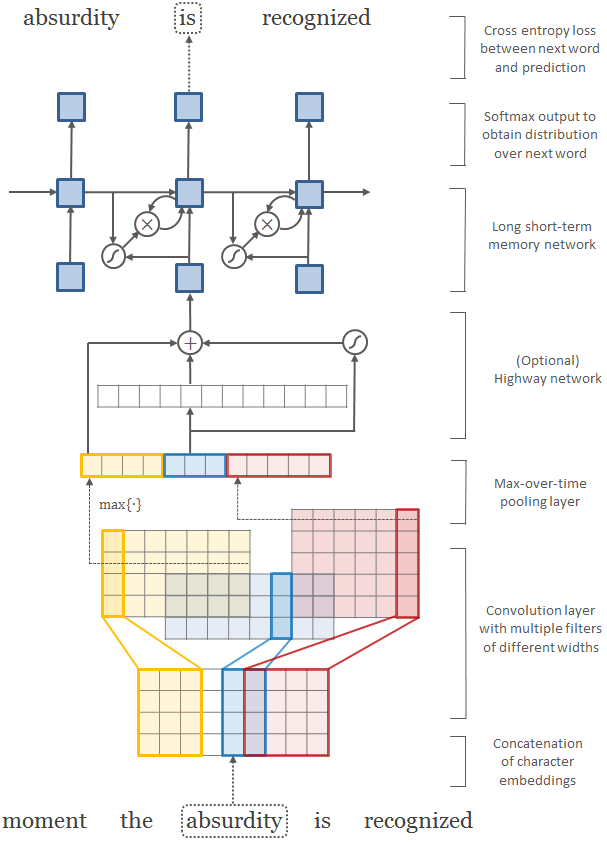
\includegraphics[width=0.4\textwidth]{network}
%  \end{center}
%\item feature tables,
%
%  \begin{center}
%    \begin{tabular}{@{}lll@{}}
%      \toprule
%      &\multicolumn{2}{c}{Mention Features  } \\
%      & Feature & Value Set\\
%      \midrule
%      & Mention Head & $\mcV$ \\
%      & Mention First Word & $\mcV$ \\
%      & Mention Last Word & $\mcV$ \\
%      & Word Preceding Mention & $\mcV$ \\
%      & Word Following Mention & $\mcV$\\
%      & \# Words in Mention & $\{1, 2, \ldots \}$ \\
%      & Mention Type & $\mathcal{T}$ \\
%      \bottomrule
%    \end{tabular}
%  \end{center}
%
%\item pseudo-code,
%
%  \begin{algorithmic}[1]
%    \Procedure{Linearize}{$x_1\ldots x_N$, $K$, $g$}
%    \State{$B_0 \gets \langle (\langle \rangle, \{1, \ldots, N\}, 0, \boldh_0, \mathbf{0})  \rangle$}
%    \For{$m = 0, \ldots, M-1$ }
%    \For{$k = 1, \ldots, |B_m|$}
%    \For{$i \in \mcR$}
%    \State{$(y, \mcR, s, \boldh) \gets \mathrm{copy}(B_m^{(k)})$}
%    \For{word $w$ in phrase $x_i$}
%    \State{$y \gets y $ append $w$ }
%    \State{$s \gets s + \log q(w, \boldh) $ }
%    \State{$\boldh \gets \delta(w, \boldh)$}
%    \EndFor{}
%    \State{$B_{m+|w_i|} \gets B_{m+|w_i|} + (y, \mcR - i, s,   \boldh)$}
%    \State{keep top-$K$ of $B_{m+|w_i|}$ by $f(x, y) + g(\mcR)$}
%    \EndFor{}
%    \EndFor{}
%    \EndFor{}
%    \State{\Return{$B_{M}^{(k)}$}}
%    \EndProcedure{}
%  \end{algorithmic}
%
%\end{itemize}


\section{Experiments}

\begin{subsection}{Trigram}
The interpolated trigram model states 
$$ p(y_{i+1}) = \alpha \cdot [p^{y_{i+1}}_{y_{i-1},y_{i}}, p^{y_{i+1}}_{y_{i}}, p^{y_{i+1}}]$$
Where $\alpha$ is a vector of length 3 with $|\alpha|_1 = 1$, and $p^a_{b}$ is the probability of word $a$ given sequence $b$ as determined by count data in the training set.\\
The unary probabilties are implemented as a vector of size $\mcV$, the binary probabilties are $\mcV \times \mcV$, and the ternary probabilties are a dictionary with keys $(w_1,w_2)$ and values vectors of size $\mcV$.\\
During training, all sequences of size 1,2 and 3 are counted. The counts are then normalized over $\mcV$. At test time, we for the most part return $\alpha \cdot p$. However, for sequences of length 1 not seen in training, we replace $p_{binary}$ with $p_{unary}$ and for sequences of length 2 not seen in training, we check if $p_{binary}$ is in training and if so use $p_{binary}$, if not use $p_{unary}$.\\
To determine the best alpha, we sample randomly from vectors of length 3 that sum to 1. We do so 5000 times and use the best one. The alpha chosen is 
$$ \alpha = [0.4306712668382596, 0.4897915705677378, 0.07953716259400256] $$
Scores for the above and other alpha of interest are reported in Table ~\ref{tab:interp}.
\begin{table}
  \begin{center}
    \begin{tabular}{@{}lll@{}}
      \toprule
      & $\alpha$ & MAP\\
      \midrule
      & [1,0,0] & 0.271 \\
      & [0,1,0] & 0.260 \\
      & [0,0,1] & 0.124 \\
      & [1/3,1/3,1/3] & 0.294 \\
      & [0.43,0.49,0.08] & 0.296\\
      \bottomrule
    \end{tabular}
  \end{center}
  \caption{\label{tab:interp} The first entry of $\alpha$ corresponds to ternary counts, and the third entry cooresponds to unary counts. The binary and ternary counts both contain considerably more information than unary.}
 \end{table}

%Word counts for positive and negative labels are all initialized to a global initial count of $\alpha$. Figure \ref{fig:clusters} shows that performance of the algorithm on the validation set is robust to changes in $\alpha$. With $\alpha=.5$, performance on the test set using binarized and count word vectors are analyzed in Table \ref{tab:nb}.\\
%The weight vector determined by Naive Bayes can be interpreted as the sentiment associated with particular words. The most positive and most negative words and their weights for binarized bag of words are shown in Table \ref{tab:nbwords}.
%
%
%
%
%
%\begin{table}[h]
%\centering
%\begin{tabular}{llrrr}
% \toprule
% Model &  & Acc. & Bce. & Roc.\\
% \midrule
% \textsc{Binarized} & & 0.791 & 0.679 & 0.867\\
% \textsc{Counts} & & 0.793  & 0.686 & 0.867\\
% \bottomrule
%\end{tabular}
%\caption{\label{tab:nb} Binarizing or counting words does not significantly affect the performance of the model on the test set.}
%\end{table}
%
%
%
%\begin{table}[h]
%\centering
%\begin{tabular}{cccccccccc}
% \midrule
% stupid & unfunny& pointless  & poorly & suffers & Feels & tiresome & car \\
%   5.39452 & 5.1085& 5.03998 &4.96641&4.96641 & 4.88701 & 4.88701 & 4.88701 \\
% \bottomrule
% \bottomrule
% powerful  & solid& perfectly & inventive & refreshing & riveting & wonderfully & universal \\
%  -5.79766 & -5.7109 & -4.99019 & -4.85754 & -4.78398 & -4.70458 & -4.61832 & -4.61832 \\
% \bottomrule
%\end{tabular}
%\caption{\label{tab:nbwords} Words with the highest and lowest weights in the naive bayes weight vector agree with intuition for being negative and positive words respectively.}
%\end{table}

\end{subsection}




\begin{subsection}{NN Language Model}
Hello


\end{subsection}

\begin{subsection}{LSTM language model}




\end{subsection}


\begin{subsection}{Embedding $\rightarrow$ Embedding}



\end{subsection}





\begin{subsection}{ResNet}



\end{subsection}






%Finally we end with the experimental section. Each assignment will make clear the main experiments and baselines that you should run. For these experiments you should present a main results table. Here we give a sample Table~\ref{tab:results}. In addition to these results you should describe in words what the table shows and the relative performance of the models.
%
%Besides the main results we will also ask you to present other results
%comparing particular aspects of the models. For instance, for word
%embedding experiments, we may ask you to show a chart of the projected
%word vectors. This experiment will lead to something like
%Figure~\ref{fig:clusters}. This should also be described within the
%body of the text itself.
%
%
%\begin{table}[h]
%\centering
%\begin{tabular}{llr}
% \toprule
% Model &  & Acc. \\
% \midrule
% \textsc{Baseline 1} & & 0.45\\
% \textsc{Baseline 2} & & 2.59 \\
% \textsc{Model 1} & & 10.59  \\
% \textsc{Model 2} & &13.42 \\
% \textsc{Model 3} & & 7.49\\
% \bottomrule
%\end{tabular}
%\caption{\label{tab:results} Table with the main results.}
%\end{table}
%
%
%\begin{figure}
%  \centering
%  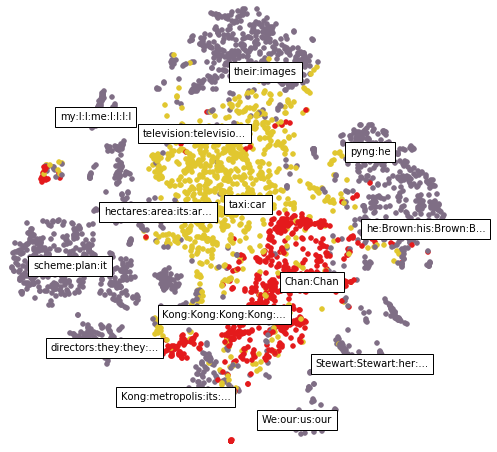
\includegraphics[width=6cm]{cluster_viz}
%  \caption{\label{fig:clusters} Sample qualitative chart.}
%\end{figure}


\section{Conclusion}

Four standard NLP models and a fifth model which has no predefined understanding of a vocabulary are trained and evaluated on SST1. The best results from all models are shown in Figure \ref{tab:conc}.

\begin{table}[h]
\centering
\begin{tabular}{llrrr}
 \toprule
 Model &  & Acc. & Bce. & Roc.\\
 \midrule
 \textsc{NB Counts} & & 0.793  & 0.686 & 0.867\\
 \textsc{Binarized LR} & & 0.789 & 0.496 & 0.876\\
 \textsc{Mean CBOW} & & 0.824 & 0.416 & 0.898\\
 \textsc{GloVe CNN} & & 0.833  & 0.577 & 0.907\\
 \midrule
 \textsc{ResNet18} & & 0.774 & 0.685 & 0.855\\
 \bottomrule
\end{tabular}
\caption{\label{tab:conc} }
\end{table}

\bibliographystyle{apalike}
\bibliography{writeup}

\end{document}
